\documentclass[12pt]{article}
\usepackage{a4wide, amsfonts, epsfig}
\newcommand\soln{\noindent\textit{Solution:} }

%NOTE that the year before has an extra inhomogeneous ode example
%
%

%skyline stuff
\font\upright=cmu10 scaled\magstep1
\setlength{\unitlength}{0.012500in}
\begingroup\makeatletter\ifx\SetFigFont\undefined
\def\x#1#2#3#4#5#6#7\relax{\def\x{#1#2#3#4#5#6}}%
\expandafter\x\fmtname xxxxxx\relax \def\y{splain}%
\ifx\x\y   % LaTeX or SliTeX?
\gdef\SetFigFont#1#2#3{%
  \ifnum #1<17\tiny\else \ifnum #1<20\small\else
  \ifnum #1<24\normalsize\else \ifnum #1<29\large\else
  \ifnum #1<34\Large\else \ifnum #1<41\LARGE\else
     \huge\fi\fi\fi\fi\fi\fi
  \csname #3\endcsname}%
\else
\gdef\SetFigFont#1#2#3{\begingroup
  \count@#1\relax \ifnum 25<\count@\count@25\fi
  \def\x{\endgroup\@setsize\SetFigFont{#2pt}}%
  \expandafter\x
    \csname \romannumeral\the\count@ pt\expandafter\endcsname
    \csname @\romannumeral\the\count@ pt\endcsname
  \csname #3\endcsname}%
\fi
\fi\endgroup

\begin{document}
\begin{center}
{\bf 2E2 Tutorial Sheet 15 Second Term, Solutions}\footnote{Conor
Houghton, {\tt houghton@maths.tcd.ie} and {\tt
http://www.maths.tcd.ie/\char126 houghton/ 2E2.html}}
\\[1cm]
 19 February 2006
\end{center}
{
Consider the non-linear differential equation
\begin{equation}
y''=y-y^2
\end{equation}
\begin{enumerate}
\item (1) By defining $y_1=y$ and $y_2=y_1'$ convert this into two first order equations.
\item (1) The stationary points are the points where $y_1'=y_2'=0$, find the two stationary points for this equation.
\item (2) Consider the $y_1=0$ stationary point, linearize the
equations near this point by assuming $y_1\ll 1$. Solve the corresponding linear equations. What sort of stationary point is this?
\item (2) Consider the $y_1=1$ stationary point, linearize the equations near this point by assuming $y_1=1+\eta$ where $\eta\ll 1$. Solve the corresponding linear equations. What sort of stationary point is this?
\item (2) Try and draw the whole phase diagram, first draw in the two
stationary points and then try and join the lines, remember the lines
don't cross.
\end{enumerate}
\vskip 1cm
\soln First we change the system into a pair of first order
equations, $y_1=y$ and
\begin{eqnarray}
y_1'&=&y_2\nonumber\\
y_2'&=&y_1(1-y_1).
\end{eqnarray}
Setting $y_1'=y_2'=0$ gives $y_2=0$ and $y_1(y_1-1)=0$ so
this has two critical points, one at $(y_1,y_2)=(0,0)$ and the second
at $(y_1,y_2)=(1,0)$. 
\vskip .5cm
Near $(0,0)$ the system linearizes to the system
\begin{eqnarray}
y_1'&=&y_2\nonumber\\
y_2'&=&y_1.
\end{eqnarray}
which has eigenvalue $\lambda_1=1$ corresponding to eigenvector
\begin{equation}
{\bf x}_1=\left(\begin{array}{c}1\\1\end{array}\right)
\end{equation}
and eigenvalue  $\lambda_1=-1$ corresponding to eigenvector
\begin{equation}
{\bf x}_1=\left(\begin{array}{c}1\\-1\end{array}\right).
\end{equation}
It is a saddlepoint. 
\vskip .5cm
Near $(1,0)$ write $y_1=1+\eta$ to get 
\begin{eqnarray}
\eta'&=&y_2\nonumber\\
y_2'&=&-\eta
\end{eqnarray}
so the eigenvalues are $\lambda=\pm i$ and the critical point is a
center.
\vskip .5cm 
To draw the phase plane, draw the saddlepoint and the
circle and try to join them up. The answer is\\ \\ \\
\begin{center}
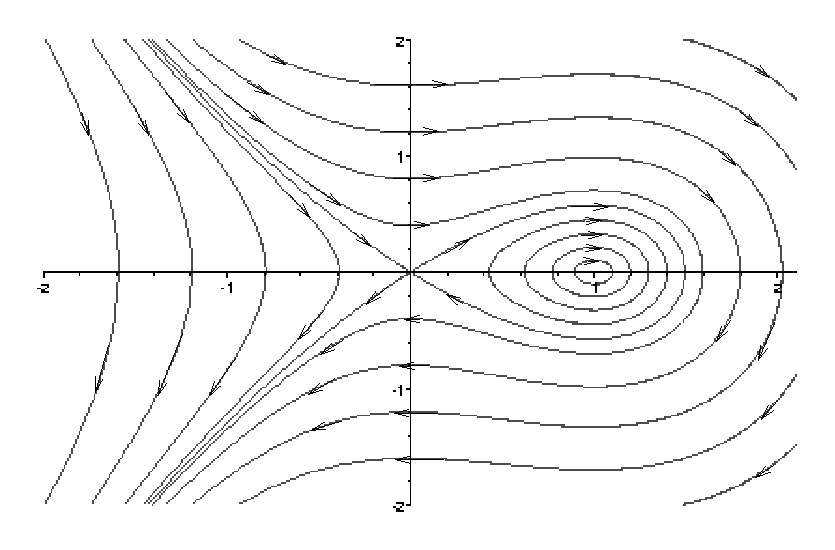
\epsfig{file=nlphase1.eps, width=12cm}
\end{center}
}
\end{document}



